\subsection{Overview}
%%%%%%%%%%%%%%%%%%%%%%%%%%%%%%%%%%%%%%%%%%%%%%%%%%%%%%%%%%
\frame {\frametitle{Cassandra: Overview (1)}
%%%%%%%%%%%%%%%%%%%%%%%%%%%%%%%%%%%%%%%%%%%%%%%%%%%%%%%%%%
\begin{itemize}
	\item {\bf Distributed key value store}
	\begin{itemize}
		\item Stores large amounts of data
		\item Linear scalability, high availability, no SPOF
	\end{itemize}

	\vspace{20pt}

	\item {\bf Tunable consistency}
	\begin{itemize}
		\item Often eventually consistent, hence in AP
		\item Can guarantee strong consistency, shifting it to CP
	\end{itemize}

	\vspace{20pt}

	\item {\bf Column-oriented data model}
	\begin{itemize}
		\item One key per row
	\end{itemize}
\end{itemize}
}

%%%%%%%%%%%%%%%%%%%%%%%%%%%%%%%%%%%%%%%%%%%%%%%%%%%%%%%%%%
\frame {\frametitle{Cassandra: Overview (2)}
%%%%%%%%%%%%%%%%%%%%%%%%%%%%%%%%%%%%%%%%%%%%%%%%%%%%%%%%%%
\begin{itemize}
	\item {\bf Combines techniques from Amazon Dynamo and HBase}
	\begin{itemize}
		\item HBase data model
		\begin{itemize}
			\item One key per row
			\item Columns, column families
		\end{itemize}
		\item Dynamo-like architecture
		\begin{itemize}
			\item Partitioning, placement (using consistent hashing)
			\item Replication, gossip-based membership, anti-entropy
		\end{itemize}
	\end{itemize}

	\vspace{20pt}

	\item {\bf Some key differences}
	\begin{itemize}
		\item Many of them recently added
	\end{itemize}
\end{itemize}
}

\subsection{Data Partitioning}
%%%%%%%%%%%%%%%%%%%%%%%%%%%%%%%%%%%%%%%%%%%%%%%%%%%%%%%%%%
\frame {\frametitle{Data Partitioning}
%%%%%%%%%%%%%%%%%%%%%%%%%%%%%%%%%%%%%%%%%%%%%%%%%%%%%%%%%%
\begin{itemize}
	\item {\bf Uses consistent hashing}
	\begin{itemize}
		\item Random Partitioner
		\item ByteOrdered Partitioner
	\end{itemize}

	\vspace{40pt}

	\item {\bf Partitioning strategy can be changed on-the-fly}
	\begin{itemize}
		\item {\color{red}All} data needs to be reshuffled
		\item Needs to be chosen carefully
	\end{itemize}
\end{itemize}
}

%%%%%%%%%%%%%%%%%%%%%%%%%%%%%%%%%%%%%%%%%%%%%%%%%%%%%%%%%%
\frame {\frametitle{Random Partitioner}
%%%%%%%%%%%%%%%%%%%%%%%%%%%%%%%%%%%%%%%%%%%%%%%%%%%%%%%%%%
\begin{itemize}
	\item {\bf Hash-based identifiers for keys (data) and storage nodes}
	\begin{itemize}
		\item Supports virtual nodes
	\end{itemize}

	\vspace{20pt}

	\item {\bf Consistent hashing + load monitoring per ring}
	\begin{itemize}
		\item Lightly loaded nodes move on the ring to alleviate heavily loaded ones
		\item Make deterministic choices about load balancing, e.g., divides the hash-ring evenly w.r.t. to number of nodes
	\end{itemize}

	\vspace{20pt}

	\item {\bf Node addition / suppression}
	\begin{itemize}
		\item Requires re-balancing the cluster if no virtual nodes
	\end{itemize}
\end{itemize}
}

%%%%%%%%%%%%%%%%%%%%%%%%%%%%%%%%%%%%%%%%%%%%%%%%%%%%%%%%%%
\frame {\frametitle{ByteOrdered Partitioner}
%%%%%%%%%%%%%%%%%%%%%%%%%%%%%%%%%%%%%%%%%%%%%%%%%%%%%%%%%%
\begin{itemize}
	\item {\bf Supports {\color{red}range queries}}
	\begin{itemize}
		\item Ensures row keys to be stored in sorted order
		\item Very different from consistent hashing
	\end{itemize}

	\vspace{20pt}

	\item {\bf Key partitioning}
	\begin{itemize}
		\item There is still a ring
		\item Keys are ordered lexicographically along the ring by their value\footnote{The key value is different from the value associated to a key}
	\end{itemize}

	\vspace{20pt}

	\item {\bf Precautions}
	\begin{itemize}
		\item Might be bad for load balancing
		\item Range scan can be obtained by using column family indexes
	\end{itemize}

\end{itemize}
}

\subsection{Data Replication}
%%%%%%%%%%%%%%%%%%%%%%%%%%%%%%%%%%%%%%%%%%%%%%%%%%%%%%%%%%
\frame {\frametitle{Data Replication}
%%%%%%%%%%%%%%%%%%%%%%%%%%%%%%%%%%%%%%%%%%%%%%%%%%%%%%%%%%
\begin{itemize}
	\item {\bf Asynchronous replication}
	\begin{itemize}
		\item Walk down the ring and choose $N-1$ successor nodes as replicas 
		\item Builds a {\color{red}preference list}
	\end{itemize}

	\vspace{20pt}

	\item {\bf Replication strategies}
	\begin{itemize}
		\item Simple Strategy:
		\begin{itemize}
			\item Main replica = node responsible for a key
			\item Additional $N-1$ replicas placed on successor nodes, clockwise in the ring, w/o rack or datacenter information
		\end{itemize}
		\item NetworkTopology Strategy
		\begin{itemize}
			\item Allows better performance when knowledge of the datacenter layout is available
			\item Reads served locally
			\item Replica placement is independent in each datacenter
			\item Rack-aware placement like in HDFS
		\end{itemize}
	\end{itemize}
\end{itemize}
}

%%%%%%%%%%%%%%%%%%%%%%%%%%%%%%%%%%%%%%%%%%%%%%%%%%%%%%%%%%
\frame {\frametitle{Data Replication Strategies: Implications}
%%%%%%%%%%%%%%%%%%%%%%%%%%%%%%%%%%%%%%%%%%%%%%%%%%%%%%%%%%
\begin{itemize}
	\item {\bf Focus on the NetworkTopology strategy}
	\begin{itemize}
		\item Requires {\color{red}Snitches}\footnote{We don't cover the details here: refer to the official documentation or the additional slides provided in the lecture notes.} and optionally Zookeeper
		\item Mechanism to discover the underlying cluster configuration
	\end{itemize}

	\vspace{24pt}

	\item {\bf Potential problems}
	\begin{itemize}
		\item Unbalanced load across datacenter
		\item Consider datacenter-specific key rings
	\end{itemize}
\end{itemize}
}

\subsection{Data Model}
%%%%%%%%%%%%%%%%%%%%%%%%%%%%%%%%%%%%%%%%%%%%%%%%%%%%%%%%%%
\frame {\frametitle{Data Model}
%%%%%%%%%%%%%%%%%%%%%%%%%%%%%%%%%%%%%%%%%%%%%%%%%%%%%%%%%%
\begin{figure}[h]
	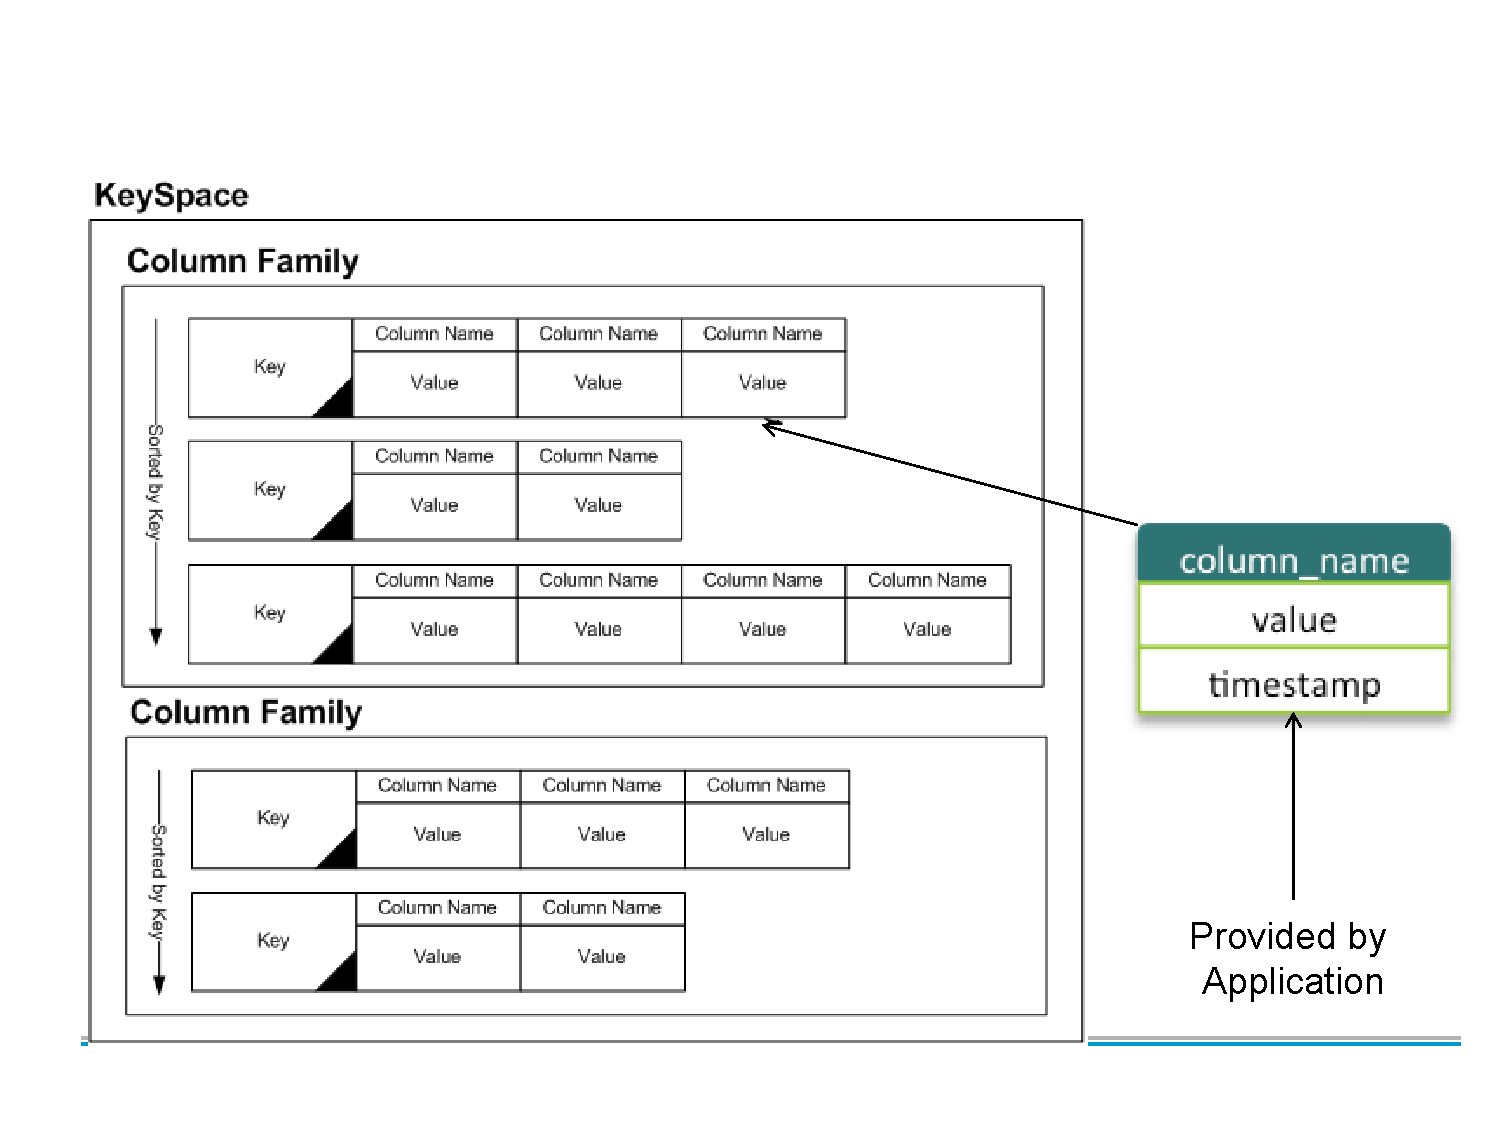
\includegraphics[scale=0.45]{./figures/cassandra_datamodel_example}
\end{figure}
}

%%%%%%%%%%%%%%%%%%%%%%%%%%%%%%%%%%%%%%%%%%%%%%%%%%%%%%%%%%
\frame {\frametitle{Data Model: Special Columns}
%%%%%%%%%%%%%%%%%%%%%%%%%%%%%%%%%%%%%%%%%%%%%%%%%%%%%%%%%%
\begin{itemize}
	\item {\bf Counter columns}
	\begin{itemize}
		\item Store counters
		\item Timestamp information automatically generated (use NTP!)
	\end{itemize}

	\vspace{20pt}

	\item {\bf Expiring columns}
	\begin{itemize}
		\item Specify a TTL value after which, data is removed
		\item Tombstone marker, as for HBase
	\end{itemize}

	\vspace{20pt}

	\item {\bf Super columns}
	\begin{itemize}
		\item Additional nesting levels
		\item Group multiple columns on a common lookup value
		\begin{itemize}
			\item E.g.: ``home address'' super column, grouping ``street'', ``city'', ``ZIP'' columns
		\end{itemize}
		\item No timestamps
	\end{itemize}
\end{itemize}
}

\subsection{Anatomy of Read/Write Operations}
%%%%%%%%%%%%%%%%%%%%%%%%%%%%%%%%%%%%%%%%%%%%%%%%%%%%%%%%%%
\frame {\frametitle{Anatomy of Read/Write Operations}
%%%%%%%%%%%%%%%%%%%%%%%%%%%%%%%%%%%%%%%%%%%%%%%%%%%%%%%%%%
\begin{itemize}
	\item {\bf Request routing}
	\begin{itemize}
		\item Proxy-based mechanism (coordinator, in Cassandra terms)
		\item Proxy route request to {\color{red}any} replica
	\end{itemize}

	\vspace{40pt}

	\item {\bf Proxy nodes}
	\begin{itemize}
		\item Handle interaction between a client and Cassandra
		\item First, determine replicas for a given key
		\item ZooKeeper may be useful here
	\end{itemize}
\end{itemize}
}

%%%%%%%%%%%%%%%%%%%%%%%%%%%%%%%%%%%%%%%%%%%%%%%%%%%%%%%%%%
\frame {\frametitle{Write Requests (1)}
%%%%%%%%%%%%%%%%%%%%%%%%%%%%%%%%%%%%%%%%%%%%%%%%%%%%%%%%%%
\begin{itemize}
	\item {\bf Proxy nodes forward write requests}
	\begin{itemize}
		\item Request routed to {\color{red}all} $N$ replicas
		\item This is true, regardless of consistency configuration
	\end{itemize}
\end{itemize}

\begin{figure}[h]
	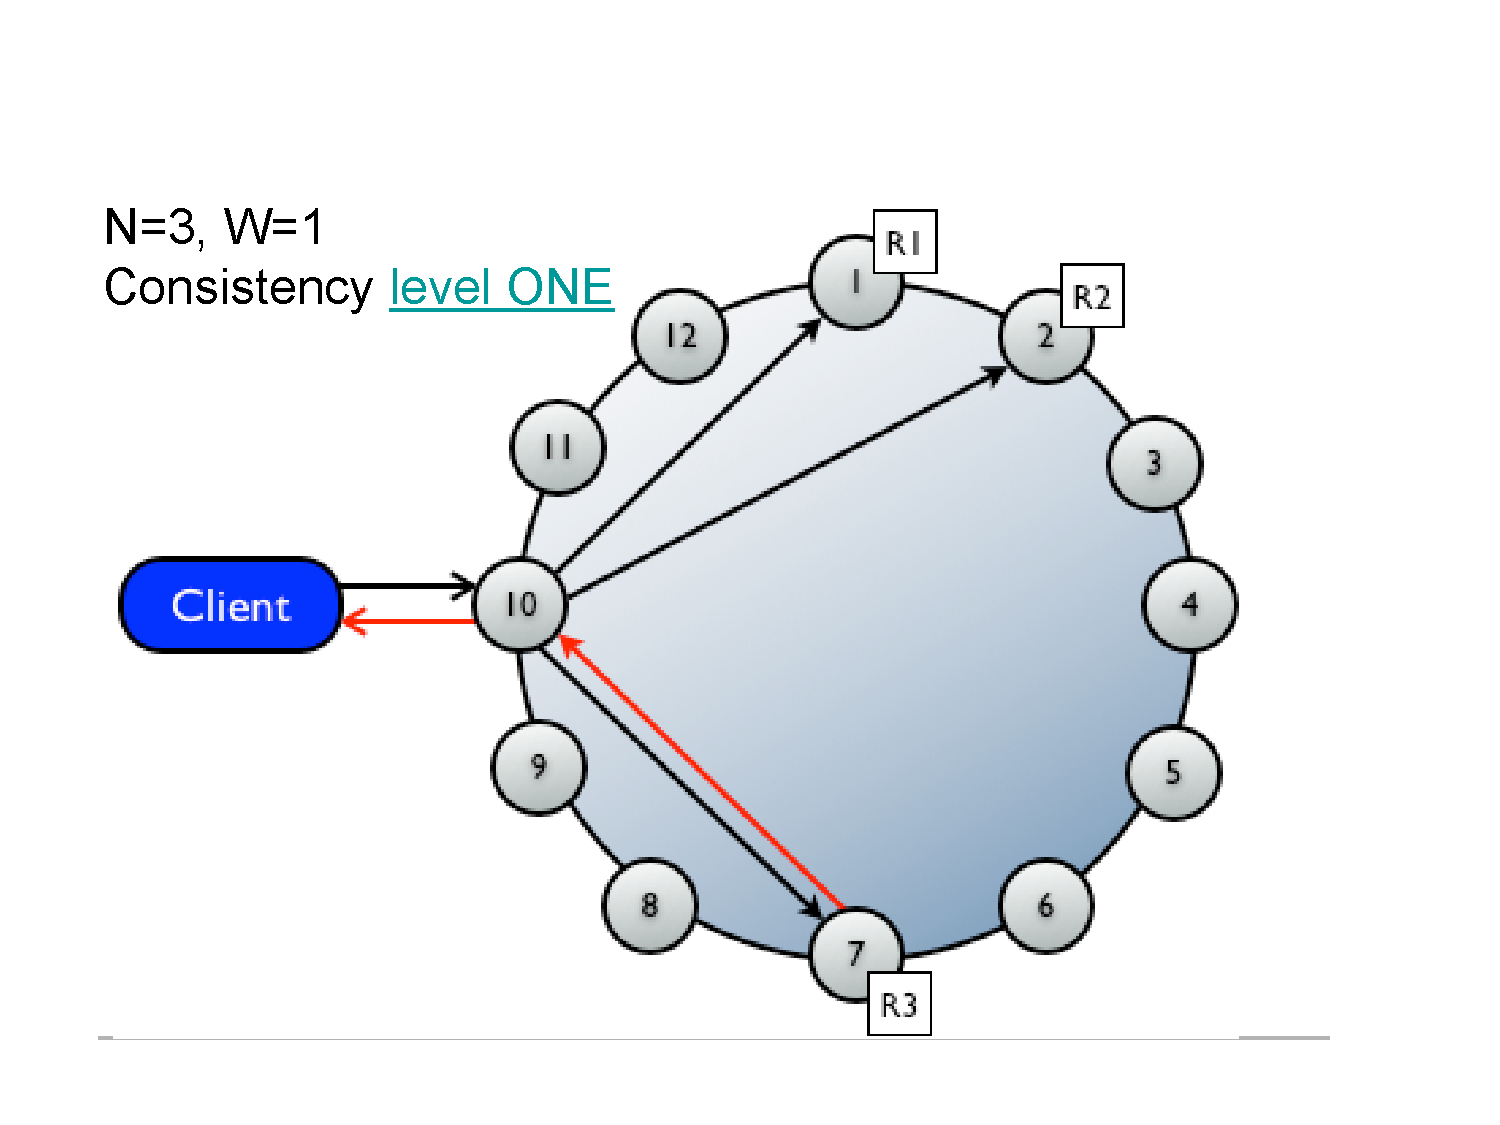
\includegraphics[scale=0.3]{./figures/cassandra_write_example}
\end{figure}
}

%%%%%%%%%%%%%%%%%%%%%%%%%%%%%%%%%%%%%%%%%%%%%%%%%%%%%%%%%%
\frame {\frametitle{Write Requests (2)}
%%%%%%%%%%%%%%%%%%%%%%%%%%%%%%%%%%%%%%%%%%%%%%%%%%%%%%%%%%
\begin{itemize}
	\item {\bf Write request}: similar mechanism to HBase
	\begin{itemize}
		\item Write to the commit log
		\item Write to in-memory data structure (\texttt{memtable})
		\item[$\to$] Write is considered successful now
		\item Writes are batched and periodically flushed to a persistent data structure called a sorted string table (\texttt{SSTable}) 
	\end{itemize}
\end{itemize}

\begin{figure}[h]
	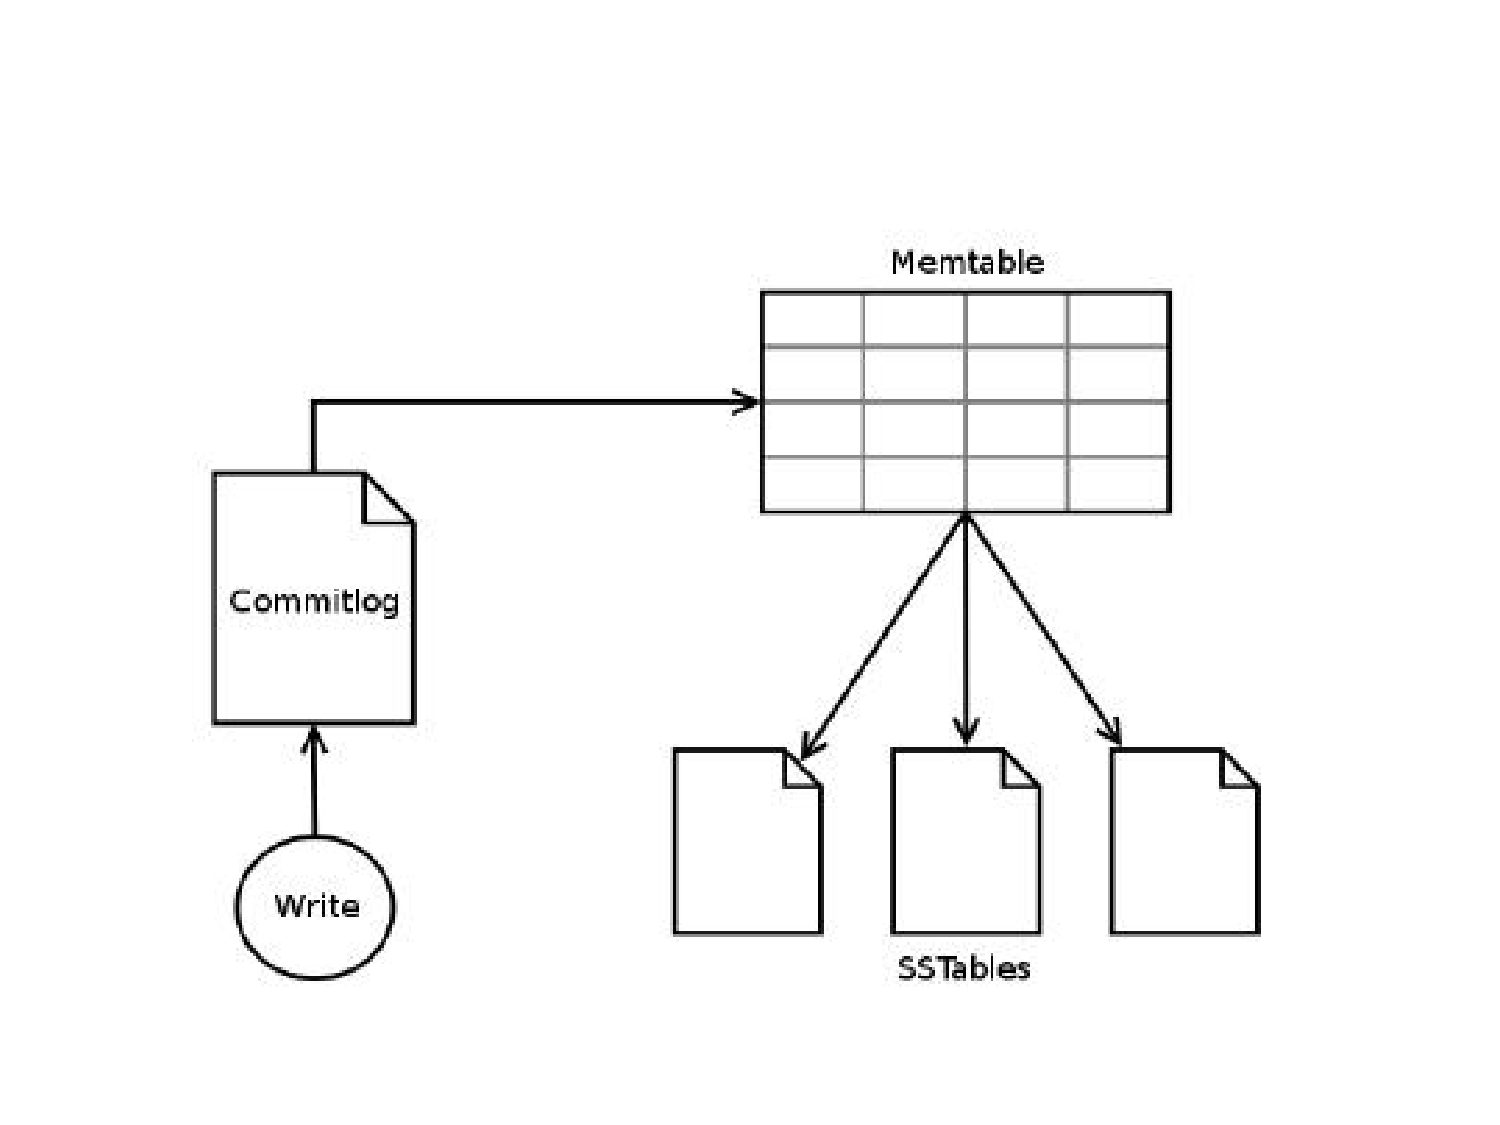
\includegraphics[scale=0.3]{./figures/cassandra_localwrite_example}
\end{figure}
}

%%%%%%%%%%%%%%%%%%%%%%%%%%%%%%%%%%%%%%%%%%%%%%%%%%%%%%%%%%
\frame {\frametitle{Write Requests (3)}
%%%%%%%%%%%%%%%%%%%%%%%%%%%%%%%%%%%%%%%%%%%%%%%%%%%%%%%%%%
\begin{itemize}
	\item {\bf Memtables}
	\begin{itemize}
		\item Organized in sorted order by row key
		\item Flushed to SSTables sequentially, no random seeks
	\end{itemize}

	\vspace{40pt}


	\item {\bf SSTables}
	\begin{itemize}
		\item Immutable (no rewrite after flushing)
		\item A single row can be stored in many SSTables
		\item[$\to$] At {\color{red}read time}, rows must be combined from all SSTables (on disk or from memtables) to produce the requested data
		\item Use {\color{red}Bloom Filters} to optimize the process
	\end{itemize}
\end{itemize}
}

%%%%%%%%%%%%%%%%%%%%%%%%%%%%%%%%%%%%%%%%%%%%%%%%%%%%%%%%%%
\frame {\frametitle{Bloom Filters (1)}
%%%%%%%%%%%%%%%%%%%%%%%%%%%%%%%%%%%%%%%%%%%%%%%%%%%%%%%%%%
\begin{itemize}
	\item {\bf Bloom Filters in a nutshell}
	\begin{itemize}
		\item Used to check for set membership
		\item $k$ hash functions hashing into the same $m$-bit space
	\end{itemize}
\end{itemize}

\begin{figure}[h]
	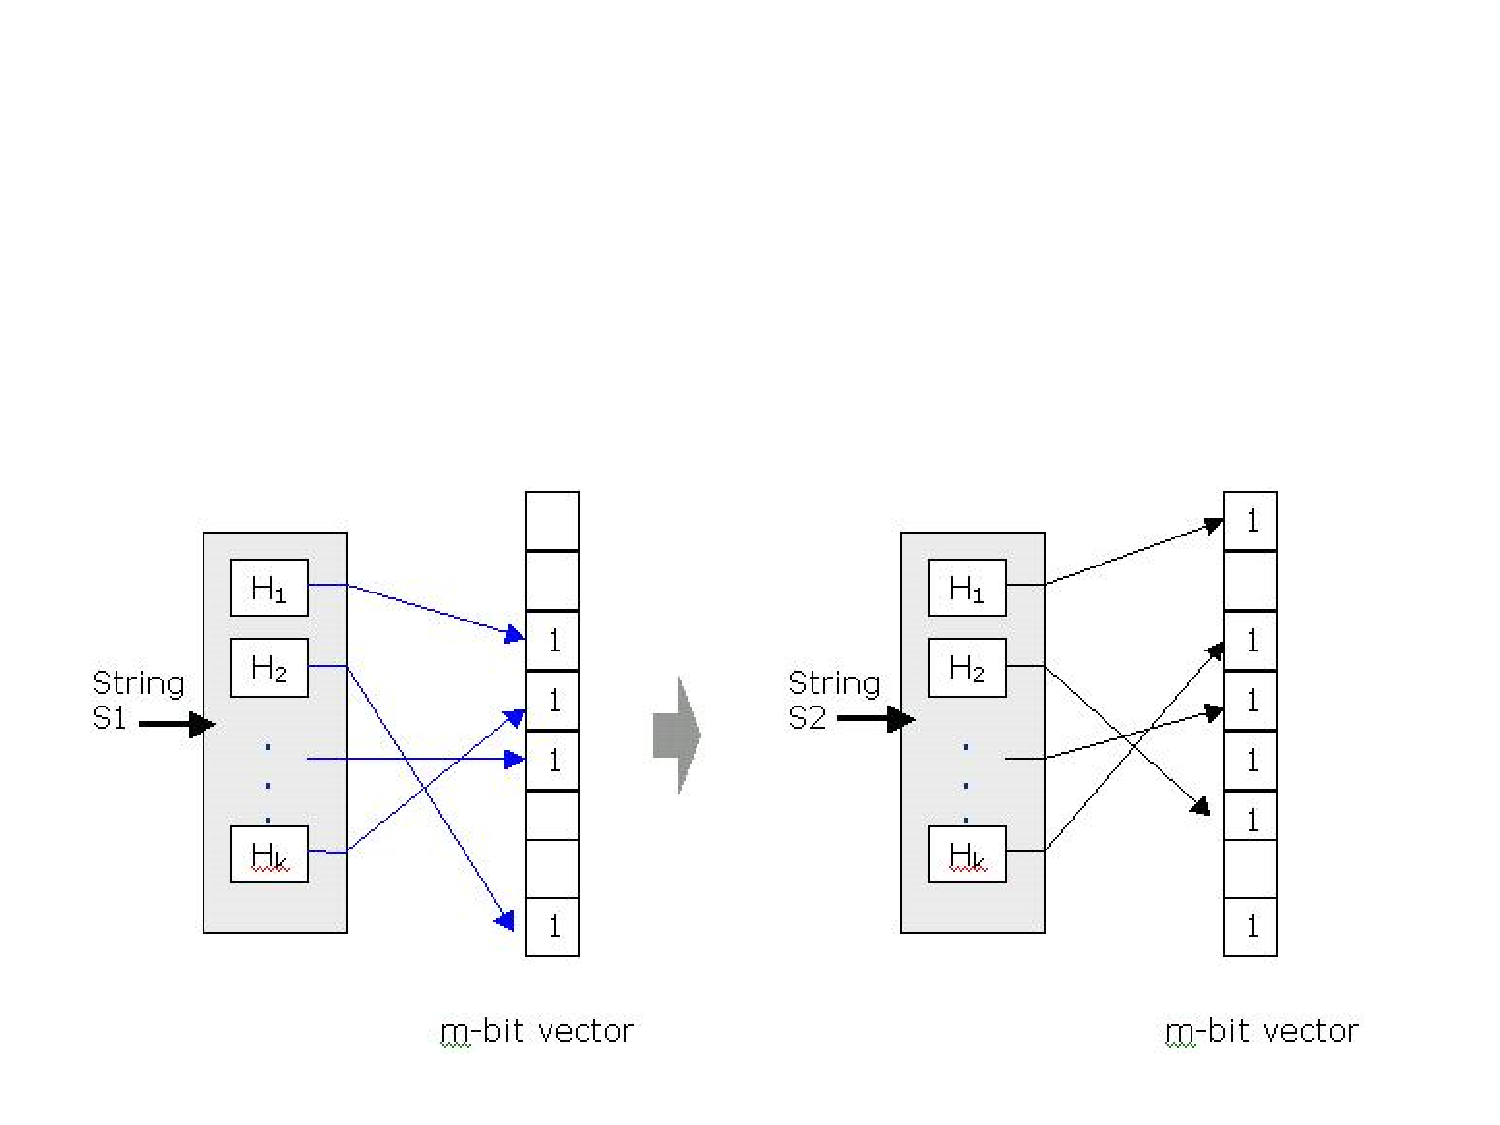
\includegraphics[scale=0.3]{./figures/cassandra_bloom_example}
\end{figure}
}

%%%%%%%%%%%%%%%%%%%%%%%%%%%%%%%%%%%%%%%%%%%%%%%%%%%%%%%%%%
\frame {\frametitle{Bloom Filters (2)}
%%%%%%%%%%%%%%%%%%%%%%%%%%%%%%%%%%%%%%%%%%%%%%%%%%%%%%%%%%
\begin{itemize}
	\item {\bf One bloom filter per SSTable}
	\begin{itemize}
		\item Used in combining from row data from multiple ``sources''
		\item Check if a requested row key exists in the SSTables, before doing any disk seeks
	\end{itemize}
\end{itemize}
\begin{figure}[h]
	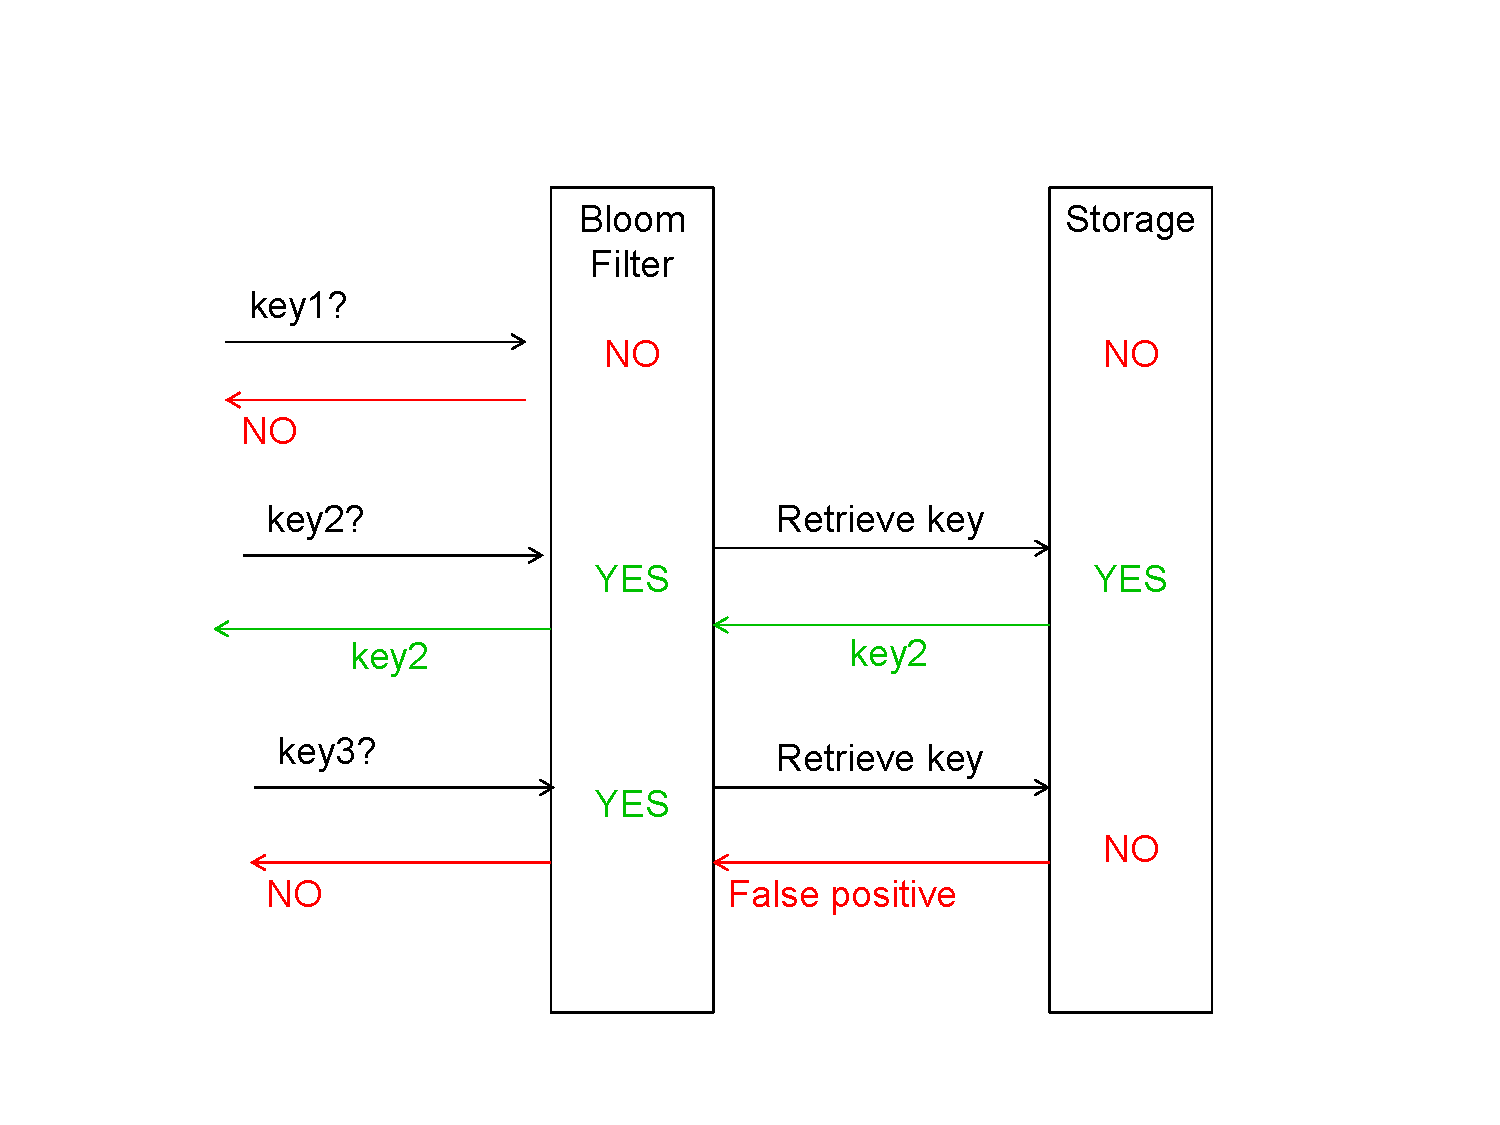
\includegraphics[scale=0.3]{./figures/cassandra_bloomrequest_example}
\end{figure}
}

%%%%%%%%%%%%%%%%%%%%%%%%%%%%%%%%%%%%%%%%%%%%%%%%%%%%%%%%%%
\frame {\frametitle{Read Requests (1)}
%%%%%%%%%%%%%%%%%%%%%%%%%%%%%%%%%%%%%%%%%%%%%%%%%%%%%%%%%%
\begin{itemize}
	\item {\bf Similar mechanism to Dynamo}
	\begin{itemize}
		\item Proxy initiates a read repair (a.k.a. writeback) if it detects inconsistent replicas
		\item This is done in the background, after the read has been served to the client
	\end{itemize}

	\vspace{40pt}

	\item {\bf The number of replicas contacted upon a read request depend on the consistency level}
	\begin{itemize}
		\item Proxy routes the requests to the closest replica
		\item Proxy routes requests to all replicas and wait for a quorum
	\end{itemize}
\end{itemize}
}

%%%%%%%%%%%%%%%%%%%%%%%%%%%%%%%%%%%%%%%%%%%%%%%%%%%%%%%%%%
\frame {\frametitle{Read Requests (2)}
%%%%%%%%%%%%%%%%%%%%%%%%%%%%%%%%%%%%%%%%%%%%%%%%%%%%%%%%%%
\begin{itemize}
	\item {\bf When a node receives a read request}
	\begin{itemize}
		\item Row must be combined from all SSTables on that node
		\item Data not yet flushed to SSTables, i.e. stored in memtables, must be considered as well
		\item[$\to$] This produces the requested data
	\end{itemize}

	\vspace{20pt}

	\item {\bf Key techniques to achieve high performance}
	\begin{itemize}
		\item Row-level column index
		\item Bloom filters
	\end{itemize}

	\vspace{20pt}

	\item {\bf Cutting read latency}
	\begin{itemize}
		\item Combining data before serving it can be slow
		\item Read cache (in memory)
		\item Advanced topics: cache invalidation, consistency...
	\end{itemize}
\end{itemize}
}


\subsection{Consistency}
%%%%%%%%%%%%%%%%%%%%%%%%%%%%%%%%%%%%%%%%%%%%%%%%%%%%%%%%%%
\frame {\frametitle{Consistency}
%%%%%%%%%%%%%%%%%%%%%%%%%%%%%%%%%%%%%%%%%%%%%%%%%%%%%%%%%%
\begin{itemize}
	\item {\bf Consistency in Cassandra is tunable}
	\begin{itemize}
		\item Hence is availability, as per CAP
		\item Read and Write consistency levels can be independent
	\end{itemize}

	\vspace{20pt}

	\item {\bf Given $N$ replicas in the preference list}
	\begin{itemize}
		\item {\color{red}Write request}: all $N$ replicas are contacted
		\begin{itemize}
			\item Ends when $W$ respond (i.e. acknowledgment)
		\end{itemize}
		\item {\color{red}Read request}: only $R$ replicas are contacted
		\begin{itemize}
			\item This is optimistic, may need to contact all $N$ replicas
		\end{itemize}
	\end{itemize}

	\vspace{20pt}

	\item {\bf Choices of $W$ and $R$ define consistency level}
	\begin{itemize}
		\item Dynamo: $W+R>N$ (recall extended preference list + sloppy quorum)
		\item Cassandra: $W+R>N$ not mandatory
	\end{itemize}
\end{itemize}
}

%%%%%%%%%%%%%%%%%%%%%%%%%%%%%%%%%%%%%%%%%%%%%%%%%%%%%%%%%%
\frame {\frametitle{Consistency Levels: ONE}
%%%%%%%%%%%%%%%%%%%%%%%%%%%%%%%%%%%%%%%%%%%%%%%%%%%%%%%%%%
\begin{itemize}
	\item {\bf $W$ = 1}
	\begin{itemize}
		\item One replica must write to commit log and memtable
	\end{itemize}

	\vspace{20pt}

	\item {\bf $R$ = 1}
	\begin{itemize}
		\item Returns a response from the closest replica (as determined by the snitch)
		\item By default, a read repair runs in the background to make the other replicas consistent
	\end{itemize}

	\vspace{20pt}

	\item {\bf This is true regardless of the replication factor $N$}
\end{itemize}
}

%%%%%%%%%%%%%%%%%%%%%%%%%%%%%%%%%%%%%%%%%%%%%%%%%%%%%%%%%%
\frame {\frametitle{Consistency Levels: QUORUM}
%%%%%%%%%%%%%%%%%%%%%%%%%%%%%%%%%%%%%%%%%%%%%%%%%%%%%%%%%%
\begin{itemize}
	\item {\bf QUORUM}
	\begin{itemize}
		\item $W=\text{floor}(N/2 + 1)$: a majority
		\begin{itemize}
			\item A write is written to the commit log and memtable on a quorum of $W$ replicas
		\end{itemize}
		\item $R=\text{floor}(N/2 + 1)$: a majority
		\begin{itemize}
			\item Read returns the record with the most recent timestamp, once a quorum of size $R$ has responded
			\item Timestamp = application timestamp
		\end{itemize}
	\end{itemize}

	\vspace{20pt}

	\item {\bf LOCAL\_QUORUM}
	\begin{itemize}
		\item Restricted to a local datacenter
	\end{itemize}

	\vspace{20pt}

	\item {\bf EACH\_QUORUM}
	\begin{itemize}
		\item QUORUM invariant must be satisfied across datacenters
	\end{itemize}
\end{itemize}
}

%%%%%%%%%%%%%%%%%%%%%%%%%%%%%%%%%%%%%%%%%%%%%%%%%%%%%%%%%%
\frame {\frametitle{Consistency Levels: ALL, ANY}
%%%%%%%%%%%%%%%%%%%%%%%%%%%%%%%%%%%%%%%%%%%%%%%%%%%%%%%%%%
\begin{itemize}
	\item {\bf ALL}
	\begin{itemize}
		\item $W=N$: all replica nodes must acknowledge
		\item $R=N$: returns the record with the most recent timestamp across all replicas
	\end{itemize}

	\vspace{40pt}

	\item {\bf ANY}
	\begin{itemize}
		\item Additional consistency for writes
		\item Allow writes to complete even if all $N$ replicas are down
		\item Hinted handoff mechanism
	\end{itemize}
\end{itemize}
}


\subsection{Lightweight Transactions}
%%%%%%%%%%%%%%%%%%%%%%%%%%%%%%%%%%%%%%%%%%%%%%%%%%%%%%%%%%
\frame {\frametitle{Lightweight Transactions}
%%%%%%%%%%%%%%%%%%%%%%%%%%%%%%%%%%%%%%%%%%%%%%%%%%%%%%%%%%
\begin{itemize}
	\item {\bf Simple mechanism at the single key level}
	\begin{itemize}
		\item Single object transactions
		\item No support for multi-key transactions
		\item ``Consistency'' level: SERIAL
	\end{itemize}

	\vspace{40pt}

	\item {\bf Compare and Swap (CAS) mechanism}
	\begin{itemize}
		\item Enhancements available in Cassandra 2.0
		\item Paxos based mechanism
		\item Address the problem of solving the agreement for 2 processes, that requires using locks
	\end{itemize}
\end{itemize}
}
